\documentclass[10pt,oneside,a4paper]{article}
\usepackage[left=2cm,right=2cm,top=2cm,bottom=1cm,includeheadfoot]{geometry}
\usepackage{ngerman}
\usepackage[utf8]{inputenc}
% \usepackage{amsfonts,amssymb,amsmath,cancel,graphicx,textcomp}
\usepackage{amsfonts,amssymb,amsmath,graphicx,textcomp}
\usepackage{float}
\usepackage{color,xcolor}
\usepackage{url}
\usepackage{hyperref}
\usepackage{listings}
\usepackage{tikz}
\usepackage{fancyhdr}
\usepackage{gensymb}
\usepackage[section]{placeins}
\usetikzlibrary{arrows,shapes,snakes,automata,backgrounds,petri,positioning}

\hypersetup{
    colorlinks,
    citecolor=black,
    filecolor=black,
    linkcolor=black,
    urlcolor=black
}

\pagestyle{fancy}
\fancyhf{}
\fancyhead[L]{crash override : \\Steve Dierker, Semjon Kerner, Artur Jeske}
\fancyhead[C]{"Ubungsblatt 11}
\fancyhead[R]{Seite \thepage}
\renewcommand{\headrulewidth}{0.5pt}

% lstlisting mit Zeilennummerierung und grauen Kommentaren, Zeilenumbruch, etc. pp.
\lstset{
  numbers=left, numberstyle=\tiny, numbersep=5pt,
  tabsize=2,
  breaklines=true, breakindent=0pt, postbreak=\mbox{$\rightarrow\ \ $},
  showstringspaces=false,
  extendedchars=false,
  basicstyle=\small\ttfamily,
  commentstyle=\color{black!40},
  stringstyle=\color{black!40!blue},
  keywordstyle=\color{black!40!green}
}

% Komma Abstände bei Tausendern/Dezimalzahlen ans dt. anpassen
\mathcode`,="013B
\setlength{\parindent}{0em}
\setlength{\parskip}{0.5em}

\begin{document}
  \section{Calculate Distance to Nearest Obstacle on Lane (10 Points)}
    \begin{figure}[h]
      \centering
      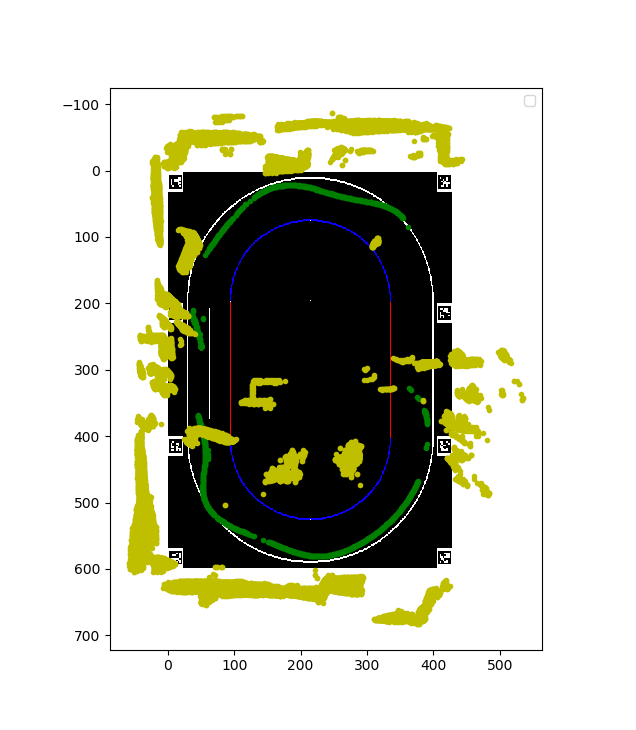
\includegraphics[scale=0.7]{pictures/circle_with_car_and_obstacles.png}
      \caption{Karte mit Lokalisationen des Autos (grün) und erkannte Objekte des LIDARs (gelb). }
    \end{figure}
    \begin{itemize}
      \item Quellcode: \url{https://github.com/bigzed/model_car/blob/version-4.0/texinput/src/localization.py}
      \item Video: \url{https://github.com/bigzed/model_car/blob/version-4.0/texinput/videos/U11_video2.MP4}
    \end{itemize}

	  Der LIDAR erkannt alle Objekte innerhalb von 1.5m vor dem Auto. `Vor dem Auto'  sind
    hierbei alle Punkte die eine positive X-Koordinate im `laser'-Koordinatensystem haben. Die
    LIDAR Daten sind kontinuierlich, allerdings ben\"otigen wir die Daten der Odometrie um sie
    in ein geminsames Koordinatensystem zu bringen. Die Transformation wird durch einen

    Wie man an den fehlenden gr\"unen Punkten im Plot erkennen kann, hat das Positionssystem
    teilweise lange Verz\"ogerugen oder wie in der Fahrt aus der der Plot stammt, kann auch eine
    komplette Kamera ausfallen. Bei dieser Fahrt war es wohl die mittlere was nach einem Neustart
    behoben war.

    Das Auto ist in dieser Fahrt ungef\"ahr an Koordinate $(80, 400)$ los gefahren und hat die
    Strecke gegen den Uhrzeigersinn befahren. Auf der rechten Gerade erkennt man die
    Ausweichbewegung um das Hindernis und auf oberen h"alfte der linken Gerade das Stoppen vor dem
    Hindernis.

    Zu beachten ist, das die anscheinend komplette Blockade der Strecke auf der rechten Seite durch
    ein nachtr"agliches Verschieben des Hindernisses von der inneren auf die \"aussere Strecke
    entstanden ist w"ahrend das Auto sich schon in der Kurve befand. Der LIDAR-Plot ist an der
    stelle irref"uhrend.
	\begin{enumerate}
    \item Für die Transformation benutzen wir \emph{tf.transformations} mit
      \emph{TransformBroadcaster} und \emph{sendTransform} und \emph{TransformListener} sowie
      \emph{transformPoint}. Die LIDAR Daten werden dann in eine \emph{PointCloud2} umgewandelt und
      durch die Transformation in das Koordinatensystem der Odomotetrie \"ubertragen.
    \item Wir benutzen die Funktion \emph{closest\_point()} von Übungsblatt 9 mit einigen Änderungen
      an der Funktion für die Bereiche im Kreis und einem leichten \emph{look ahead}.\\
      Der Lenkeinschlag wird aus dem Winkeln zwischen Orientierung des Autos und dem Vektor vom Auto
      zum \emph{closest\_point} bestimmt. Diesen Winkel nehmen als Fehler fuer einen KP-Kontroller
      den Lenkwinkel bestimmt.
    \item In unserer \emph{lane\_is\_free} Funktion wird f\"ur jedes erkannte Hindernis
      des LIDARs getestet ob es auf der derzeitigen Spur liegt, falls nicht behalte die Spur bei.

      Falls ein Hindernis auf dieser Spur ist, \"uberpr\"ufe die andere und falls diese frei ist,
      wechsle die Spur. Sollte diese ebenfalls belegt sein halten wir an, bis eine der Spuren wieder
      frei wird.
	\end{enumerate}
\end{document}
